\subsection{Análisis cualitativo}

El objetivo de esta sección es plantear y responder preguntas que nos lleven a entender mejor CMM y a encontrar ventajas y desventajas del mismo. Para ello primeramente propondremos casos pequeños, que no necesariamente representan casos de competencias reales.

\subsubsection{Planteo de casos}

\subsubsection*{Caso 1}
Se inicia un sistema con dos equipos: 1, y 2, con un único partido entre ellos: 1 vs 2 a favor de 1.

\textbf{Pregunta}: ¿Qué pasará con los ratings? ¿Hay alguna relación entre ellos?

\begin{table}[h!]
    \begin{center}
        \begin{tabular}{|c|c|c|}
        \hline
        \textbf{Posición} & \textbf{Equipo} & \textbf{Rating} \\
        \hline
        1 & 1 & 0.625\\
        2 & 2 & 0.375\\
        \hline
        \end{tabular}
        \caption{Ranking CMM luego de iniciar un partido 1 vs 2, a favor de 1}
        \label{cmm_caso_1}
    \end{center}
\end{table}

\textbf{Observación}: Acorde a la \textit{Regla de Laplace de sucesos} utilizar el estimador planteado por la misma nos permite que no hayan cambios abruptos en la resolución de los ratings de los equipos involucrados.

\subsubsection*{Caso 2}

Sobre el sistema anterior: se agregan cinco partidos a favor de 1.

\textbf{Pregunta}: ¿Qué pasará con los ratings? ¿Hay alguna relación entre ellos?

\begin{table}[h!]
    \begin{center}
        \begin{tabular}{|c|c|c|}
        \hline
        \textbf{Posición} & \textbf{Equipo} & \textbf{Rating} \\
        \hline
        1 & 1 & 0.714286\\
        2 & 2 & 0.285714\\
        \hline
        \end{tabular}
        \caption{Ranking CMM luego de cinco partidos 1 vs 2, a favor de 1}
        \label{cmm_caso_2}
    \end{center}
\end{table}

\textbf{Observación}: Los ratings se ajustan acorde a los resultados de los partidos. Como vimos hasta ahora, los mismos dependen de la cantidad de partidos que hayan entre los equipos competidores.

\subsubsection*{Caso 3}

Sobre el sistema anterior: se suma un equipo, 3. 3 vs 2 a favor de 3.

\textbf{Pregunta}: ¿Será mejor el rating de 3 que el de 2?

\begin{table}[h!]
    \begin{center}
        \begin{tabular}{|c|c|c|}
        \hline
        \textbf{Posición} & \textbf{Equipo} & \textbf{Rating} \\
        \hline
        1 & 1 & 0.68\\
        2 & 3 & 0.58\\
        3 & 2 & 0.24\\
        \hline
        \end{tabular}
        \caption{Ranking CMM luego de introducir a 3 y agregar un partido a favor de 3}
        \label{cmm_caso_3}
    \end{center}
\end{table}

\textbf{Observación}: Después de 3 vs 2 a favor de 3, 3 supera fácilmente a 2 modificando sus posiciones. El rating de 2 desciende esperadamente, pero el de 1 también aunque sigue manteniendo su posición. Al no estar 1 involucrado en este partido, vemos que CMM afecta el rating (y tal vez el ranking) de equipos que no formaron parte del partido.

\newpage

\subsubsection*{Caso 4}

Sobre el sistema anterior: se agregan diez partidos, 3 vs 2 a favor de 3.

\textbf{Pregunta}: ¿Se acercará el rating de 3 al rating de 1?

\begin{table}[h!]
    \begin{center}
        \begin{tabular}{|c|c|c|}
        \hline
        \textbf{Posición} & \textbf{Equipo} & \textbf{Rating} \\
        \hline
        1 & 3 & 0.662963\\
        2 & 1 & 0.644444\\
        3 & 2 & 0.192593\\
        \hline
        \end{tabular}
        \caption{Ranking CMM luego de agregar diez partidos a favor de 3}
        \label{cmm_caso_4}
    \end{center}
\end{table}

\textbf{Observación}: En este caso se ve que CMM permite alterar no solo el rating, si no la posición de los equipos, ya que 3 vs 1 nunca tuvo lugar. Esto de alguna forma nos habla de "la justicia del método": ¿es justo que 1 descienda si nunca se enfrentó con 3?. Claramente la relación entre ambos equipos viene dada por los partidos que tuvieron de forma separada con 2. 1 vs 2 se dió hasta ahora seis veces mientras que 3 vs 2 se dió hasta ahora once veces.

\subsubsection*{Caso 5}

Sobre el sistema anterior: se agregan cinco partidos, 1 vs 2 a favor de 1.

\textbf{Pregunta}: Si la relación entre 1 y 3 es intermediada por la cantidad de partidos que ambos ganaron a 2, ¿será cierto que ambos tendrán el mismo rating si igualan la cantidad de partidos con 2?

\begin{table}[h!]
    \begin{center}
        \begin{tabular}{|c|c|c|}
        \hline
        \textbf{Posición} & \textbf{Equipo} & \textbf{Rating} \\
        \hline
        1 & 1 & 0.657143\\
        1 & 3 & 0.657143\\
        2 & 2 & 0.185714\\
        \hline
        \end{tabular}
        \caption{Ranking CMM luego de que 1 y 3 obtengan la misma configuración de partidos}
        \label{cmm_caso_5}
    \end{center}
\end{table}

\textbf{Observación}: En este caso se ve que a igual cantidad de partidos ganados de 1 y 3 vs 2, se obtiene el mismo rating.

\subsubsection*{Caso 6}

Sobre el sistema anterior: se suma un equipo, 4. 4 vs 3 a favor de 4.

\textbf{Pregunta}: ¿Qué pasará si un nuevo equipo tiene un partido contra el equipo que está en la primera posición?

\begin{table}[h!]
    \begin{center}
        \begin{tabular}{|c|c|c|}
        \hline
        \textbf{Posición} & \textbf{Equipo} & \textbf{Rating} \\
        \hline
        1 & 4 & 0.692159\\
        2 & 1 & 0.606041\\
        3 & 3 & 0.576478\\
        4 & 2 & 0.125321\\
        \hline
        \end{tabular}
        \caption{Ranking CMM luego de agregar al sistema anterior un nuevo equipo con un partido a favor}
        \label{cmm_caso_6}
    \end{center}
\end{table}

\textbf{Observación}: En un solo partido, 4 llegó a la primera posición. Se puede explicar que 1 haya quedado por arriba de 3 ya que la configuración de partidos jugados es un factor que está presente en CMM: 4 vs 3 deja a 3 con un partido más, pero perdido, a diferencia de 1 que no sumó partidos.

\newpage

\subsubsection*{Caso 7}\label{caso_7}

Sobre el sistema anterior: se agregan cien partidos, 2 vs 3 a favor de 2.

\textbf{Pregunta}: ¿Puede alcanzar 2 las primeras posiciones si gana partidos contra los equipos de las últimas posiciones?

\begin{table}[h!]
    \begin{center}
        \begin{tabular}{|c|c|c|}
        \hline
        \textbf{Posición} & \textbf{Equipo} & \textbf{Rating} \\
        \hline
        1 & 1 & 0.905919\\
        2 & 4 & 0.52859\\
        3 & 2 & 0.479722\\
        4 & 3 & 0.0857696\\
        \hline
        \end{tabular}
        \caption{Ranking CMM luego de agregar cien partidos a favor de 2}
        \label{cmm_caso_7}
    \end{center}
\end{table}

\textbf{Observación}: Se observa que por un lado 2 y 3 intercambiaron posiciones, lo que muestra que, aunque los ajustes de rating se hagan con cada partido, los máximos valores que pueden tener se ven limitados a los valores de los equipos que se enfrentaron. Por otro lado 1 y 4 intercambiaron lugares también: esto puede deberse a que hasta este momento 3 y 4 se enfrentaron en una ocasión a favor de 4, es probable que su caída en el puesto sea debido a la caída de 3 (su victoria se desprestigia).

\subsubsection*{Caso 8}

Sobre el sistema anterior: se agregan tantos partidos como sea necesario para desplazar a 1 de la primera posición, 3 vs 1 a favor de 3.

\textbf{Pregunta}: Estando 3 en la última posición, ¿se podrá desplazar a 1 de la primera posición en pocos partidos?

\begin{table}[h!]
    \begin{center}
        \begin{tabular}{|c|c|c|}
        \hline
        \textbf{Posición} & \textbf{Equipo} & \textbf{Rating} \\
        \hline
        1 & 2 & 0.597924\\
        2 & 4 & 0.583805\\
        3 & 1 & 0.566854\\
        4 & 3 & 0.251416\\
        \hline
        \end{tabular}
        \caption{Ranking CMM luego de siete partidos 3 vs 1 a favor de 3}
        \label{cmm_caso_8}
    \end{center}
\end{table}

\textbf{Observación}: En siete partidos, 3 fue capaz mediante CMM de que 2 reemplazara a 1 en el primer lugar. ¿Por qué 2 y no 4? Es probable que sea debido a la cantidad de partidos 1 vs 2 que se hayan dado.

\subsubsection*{Caso 9}\label{caso_9}

Sobre el sistema del caso 7 \ref{caso_7}: se agregan tantos partidos como sea necesario para desplazar a 1 de la primera posición, 3 vs 2 a favor de 3.

\textbf{Pregunta}: Estando 3 en la última posición, ¿se podrá desplazar a 1 de la primera posición en pocos partidos?

\begin{table}[h!]
    \begin{center}
        \begin{tabular}{|c|c|c|}
        \hline
        \textbf{Posición} & \textbf{Equipo} & \textbf{Rating} \\
        \hline
        1 & 1 & 0.858055\\
        2 & 4 & 0.554697\\
        3 & 2 & 0.423156\\
        4 & 3 & 0.164091\\
        \hline
        \end{tabular}
        \caption{Ranking CMM luego de veinte partidos 3 vs 2 a favor de 3}
        \label{cmm_caso_9}
    \end{center}
\end{table}

\textbf{Observación}: En veinte partidos, 3 aún no fue capaz mediante CMM de que un equipo reemplazara a 1 en el primer lugar.

\newpage
\subsubsection{¿Qué podemos decir sobre CMM en base a las observaciones?}\label{conclusion_observaciones}

Estos ejemplos sencillos nos permitieron entender un poco más CMM a la hora de rankear equipos.

Desde el caso 1 al caso 5, probamos introducir un equipo y hacerlo avanzar compitiendo con el equipo de la última posición. Vimos que puede alcanzar un mejor puesto en el ranking tratando de obtener una configuración similar a la de los equipos que están en la posición deseada, lo cual es esperado para un ranking en general. Vimos también que el resultado de un partido influye sobre otros equipos mediante una "transitividad" (caso 4).

Desde el caso 6 al caso 9, quisimos hacer foco en como un equipo puede avanzar en la tabla. Ingresamos un participante más a nuestro sistema, dejando un total de cuatro y volviéndolo un poco más complejo, corroboramos que los equipos son susceptibles a cambios en su rating si algún equipo con el que tuvo relación tiene un partido. Por otra parte, notamos que un equipo en la tabla avanza más lento conforme se enfrenta a equipos que están en las últimas posiciones y más rápido conforme se enfrenta a otros que está en las primeras:

\begin{itemize}
    \item en el caso 7: 3 vs 2, favor a 3. Después de cien partidos 2 había avanzado una posición.
    \item en el caso 8: 3 vs 1, favor a 3. En siete partidos se logra que 2 desplace a 1.
    \item en el caso 9: 3 vs 2, favor a 3. En veinte partidos no se logró mover a 1 del primer lugar.
\end{itemize}

Tiene sentido esto último ya que tal vez pueda considerarse que no hay suficiente mérito en vencer a equipos que están en las últimas posiciones.

\subsubsection{Interpretación del sistema $Cr = b$ y una explicación a las observaciones}\label{interpretacion_sistema}

Como se desarrolla en \cite{CMMpaper}, la solución al sistema $Cr = b$ son los ratings de los equipos involucrados en la competencia. Saliendo de su expresión matricial, obtenemos que para un equipo $e_i \in \{e_1, \dots, e_n\}$:

\begin{equation}
    r_i = \frac{1 + \frac{w_i - l_i}{2} + \sum_{j=1, j \neq i}^{n}{n_{i,j} * r_j}}{2 + n_i}    
\end{equation}

donde para $e_k$:

\begin{itemize}
    \item $r_k$ es el rating buscado
    \item $w_k$ es la cantidad de partidos ganados
    \item $l_k$ es la cantidad de partidos perdidos
    \item $n_k$ es la cantidad de partidos jugados
    \item $n_{k,l}$ es la cantidad de partidos jugados entre $e_k$ y $e_l$ 
\end{itemize}

La primera observación que podemos hacer es que conforme aumente la cantidad de partidos, \textbf{el denominador principal aumenta}, con lo cual \textbf{$r_i$ se vuelve más pequeño}.\\

En segundo lugar, hay dos términos en el numerador principal que contribuyen a aumentar o disminuir $r_i$:

\begin{itemize}
    \item $\frac{w_i - l_i}{2}$: Alcanza su valor más alto cuando se ganan todos los partidos, contrariamente, es muy desventajoso si se pierden más partidos de los que se ganan dado que se vuelve negativo. En general, del numerador principal, representa la mayor parte del valor de $r_i$. Observemos también que a medida que este valor cambia, el denominador principal aumenta, por lo que la \textbf{ventaja máxima se encuentra ganando partidos}.
    \item $\sum_{j=1, j \neq i}^{n}{n_{i,j} * r_j}$: Es una suma en la que cada en cada término se encuentra la cantidad de partidos disputados entre $e_i$ y $e_j$ ponderado por $r_j$. Cada término de la suma \textbf{aporta tanto como $n_{i, j}$ cuando $r_j$ tiene un valor cercano a $1$} y aporta menos cuando el mismo tiene un valor cercano a $0$.
\end{itemize}

\newpage
Esto nos permite explicar el carácter ``transitivo'' de CMM: partidos de equipos con los que $e_i$ haya jugado impactarán en uno de los términos de la última sumatoria vista de forma proporcional a la cantidad de partidos disputados entre $e_i$ y el equipo en cuestión.

\subsubsection{Una estrategia para avanzar en el ranking minimizando la cantidad de partidos}\label{estrategia}

En base a la interpretación anterior, podemos sacar ventaja de CMM si:

\begin{itemize}
    \item Se compensa la relación entre los términos $(2 + n_i)$ y $\frac{w_i - l_i}{2}$ para evitar que $r_i$ disminuya. Esto se logra manteniendo al máximo la cantidad de partidos ganados.
    \item De ser posible, jugar menos partidos que los demás equipos.
    \item Teniendo en cuenta el carácter transitivo mencionado previamente, jugar uniformemente con equipos que tengan bajo rating (dado que la probabilidad de ganarles es mayor) una cantidad considerable de partidos, mientras más, mejor. Eventualmente en la intención de llegar a mejores posiciones de estos equipos, alguno (o ninguno) empezará a subir en la tabla impactando proporcionalmente a la cantidad de partidos que haya jugado con el equipo que aplique la estrategia. También se puede jugar siempre con un mismo equipo de rating bajo, pero la posibilidad de encontrar una ventaja se limita a qué tan bien le vaya a ese único equipo.
\end{itemize}

\subsubsection{¿Es CMM un método justo?}

Puede pasar que el rating de un equipo se vea afectado por una partida en la que no estuvo involucrado.

Sabemos que de poder elegir contra quien y cuantos partidos jugar, un equipo puede plantear una estrategia para subir su rating sin haber jugado como los otros.

En el caso 9 \ref{caso_9} presentado en la sección anterior. se observa que si un equipo que está en las últimas posiciones quiere llegar al primer lugar, es difícil que lo haga ganando partidas con equipos que están en posiciones más bajas o bien que no tienen relación alguna con los equipos que están por encima del que quiere subir. Aún después de haber jugado, como en ese caso más de veinte partidos. Por eso también aplicar la estrategia mencionada previamente puede ser arriesgada.

En base a estas cosas, podría calificarse a CMM como un método \textbf{no  justo, de no tener la competencia reglas claras} que determinen la forma de juego, asegurando que no se puedan incurrir en tales estrategias o asegurando que todos jueguen contra todos. Cabe destacar que en este último caso CMM pierde un poco de gracia y un rankeo por medio de puntos (como en fútbol por ejemplo) sería más efectivo.

%--------------------------------------------------------
\FloatBarrier
\subsection{CMM y otros algoritmos de rankeo}\label{cmm_comparacion}
En la tabla \ref{tab:tops10CMM} se puede ver los nombres de los tenistas en el top 10 de CMM, a modo informal de comparación agregamos su posición en WP y Elo así como también su ranking ``real''\footnote{Según \url{https://www.atptour.com/en/rankings/singles?rankDate=2015-12-28&rankRange=0-100}}. CMM hace un gran trabajo ``descubriendo'' cuales son los jugadores top 10, faltando solo uno del ranking oficial (Jo-Wilfried Tsonga) aunque mezcla un poco las posiciones.

\begin{table}
\centering
\begin{tabular}{|l|l|l|c|c|c|c|}
\hline
id&first\_name&last\_name&CMM\_rank&Elo\_rank&WP\_rank&Ranking\_real\\
\hline
104925&Novak&Djokovic&1&1&27&1\\
\hline
103819&Roger&Federer&2&2&28&3\\
\hline
104918&Andy&Murray&3&3&31&2\\
\hline
104527&Stanislas&Wawrinka&4&6&41&4\\
\hline
105453&Kei&Nishikori&5&5&34&8\\
\hline
104745&Rafael&Nadal&6&4&35&5\\
\hline
104607&Tomas&Berdych&7&9&42&6\\
\hline
103970&David&Ferrer&8&7&33&7\\
\hline
104755&Richard&Gasquet&9&8&43&9\\
\hline
105683&Milos&Raonic&10&12&45&14\\
\hline
\end{tabular}
\caption{Posiciones de top 10 de CMM en otros rankings.}
\label{tab:tops10CMM}
\end{table}






Más allá de estos datos curiosos vamos a ver la relación lineal entre CMM y los demás rankings, usando scatterplots, coeficiente de Pearson y \textit{Kendall’s weighted $\tau$}. Este último lo descubrimos buscando métodos para comparar rankings, según entendemos es un algoritmo bastante usado y es parte del conjunto de funciones de \href{https://docs.scipy.org/doc/scipy/reference/generated/scipy.stats.weightedtau.html}{Scipy}.

Según se explica tanto en la documentación oficial de Scipy como en el paper que presenta la idea \cite{kendall} el algoritmo compara los rankings dando más importancia a los valores de mayor magnitud, pero teniendo en cuenta aún los más chicos. La explicación matemática de cómo se realiza queda fuera de nuestro alcance por el momento aunque nos gustaría verla en detalle de ser posible.

Analizaremos estos algoritmos de rankeo utilizando el conjunto de datos de partidos de ATP 2015\cite{repoAtp}.

%--------------------------------------------------------
\FloatBarrier
\subsubsection{Porcentaje de victorias}

En la figura \ref{fig:sc_cmm_wp} podemos ver que la correlación lineal entre CMM y WP es bastante buena salvo por unos grupos de outliers. El coeficiente de Pearson es 0.805, mostrando que esos grupos de outliers no afectan \textit{tanto} y la relación es cercana. Por otro lado el coeficiente de Kendall es 0.763, un poco más bajo lo que indicaría, si mal no entendemos, que la relación no es tan buena para los primeros puestos. Esto concuerda en principio con la tabla \ref{tab:tops10CMM} presentada al comienzo.

\begin{figure}[h]
 \centering
 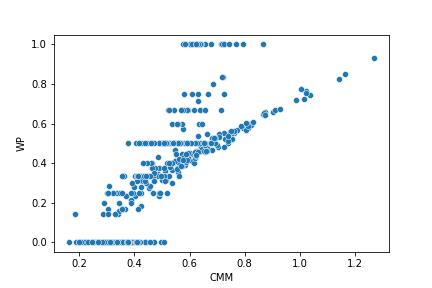
\includegraphics[scale=0.8]{imagenes/scatterplot_CMM_WP.png}
 \caption{Correlación lineal entre CMM y WP}
 \label{fig:sc_cmm_wp}
\end{figure}

En cuanto a los tres grupos principales de outliers podemos ver que se tratan de los que tienen WP = 0, 0.5 y 1. Al no tener el ajuste de la regla de Laplace si no se ganó/perdió algún partido los valores van a parar a uno de los extremos; además si se tiene la misma cantidad de ganadas que perdidas el valor de WP será 0.5 ya que no considera ``fuerza'' del adversario.\\

Previamente analizamos la composición de $r_i$ para CMM, ahora vamos a analizarla para WP y asi entender las similitudes que se observan.

Para el algoritmo WP:

\begin{equation}
    r_i = \frac{w_i}{n_i}   
\end{equation}

donde $w_i$ y $n_i$ tienen el mismo significado que para la definición de CMM \ref{interpretacion_sistema}.

Es importante recordar que la definición de CMM tiene su origen en una variación de WP, utilizando la Regla de Laplace de sucesos. Por lo que:

\begin{equation}
    r_i = \frac{1 + \frac{w_i - l_i}{2} + \sum_{j=1, j \neq i}^{n}{n_{i,j} * r_j}}{2 + n_i} = \frac{1 + w_i}{2 + n_i}
\end{equation}

si se toma la igualdad $w_i = \frac{w_i - l_i}{2} + \frac{n_i}{2}$, asumiendo que todos los equipos inician el sistema con $r_i = \frac{1}{2}$.

Observemos que al final, la expresión de $r_i$ para CMM es muy parecida a la expresión de $r_i$ para WP, por lo que es esperable un comportamiento similar, siempre teniendo en cuenta que el estimador que es objeto de estudio en este trabajo, tiene como objetivo aportar coherencia al asignar ratings y en eso difieren.

%--------------------------------------------------------
\FloatBarrier
\subsubsection{Elo}

Elo y CMM se parecen menos linealmente, como se puede ver en la figura \ref{fig:sc_cmm_elo}. Su coeficiente de Pearson es 0.789, un poco menos que con WP. Mientras que su coeficiente de Kendall es 0.868, esto nos indica que, si bien no son muy parecidos linealmente tienden a rankear de manera similar los jugadores con mayor cantidad de ``puntaje''. Esto también concuerda con la tabla \ref{tab:tops10CMM} de tops.

\begin{figure}[h]
 \centering
 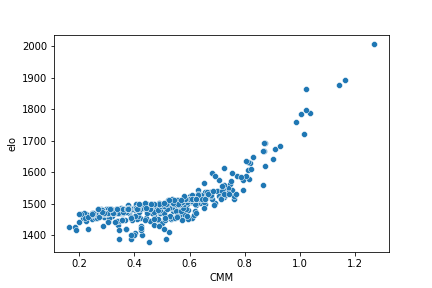
\includegraphics[scale=0.8]{imagenes/scatterplot_CMM_Elo.png}
 \caption{Correlación lineal entre CMM y Elo}
 \label{fig:sc_cmm_elo}
\end{figure}

De la misma forma que en la sección anterior, pasamos a analizar el cálculo de Elo para entenderlo mejor.

Elo se compone de dos partes:

\begin{itemize}
    \item La probabilidad de que un equipo $e_i$ gane sobre un equipo $e_j$: $p(elo_i, elo_j) = \frac{1}{1 + 10^{\frac{elo_j - elo_i}{400}}}$
    \item Actualización del rating Elo de un equipo $e_i$ que se enfrentó a un equipo $e_j$: $u(elo_i, elo_j, p_i) = elo_i + k(p_i - p(elo_i, elo_j))$ donde $p_i$ es el puntaje que hizo el equipo $e_i$ en el partido y $k$ es un coeficiente de actualización, fija en tiempo de implementación, que entre otras cosas determina cuantos puntos se ganan o se pierden como máximo.
\end{itemize}

Algunas diferencias respecto a CMM que se pueden deducir en base a lo mencionado:

\begin{itemize}
    \item La actualización de $elo_i$ sólo depende del equipo contrincante y de su rating elo ($elo_j$). Por lo que no hay influencia sobre otros equipos.
    \item Hasta $k$ puntos puede avanzar o retroceder $elo_i$ dependiendo del resultado del partido y de qué tan probable sea que un equipo gane a otro. Los equipos con resultados más inesperados (a favor o en contra) son los que reciben la mayor diferencia.
    \item En base a lo anterior, es poco ventajoso que equipos fuertes se enfrenten a equipos débiles dado que en esos partidos la ganancia de puntos en el ranking es mínima.
    \item Se entiende a Elo como un sistema que permite medir el progreso, dado que recompensa o penaliza las sorpresas.
\end{itemize}
